%\VignetteEngine{knitr::knitr}
%\VignetteIndexEntry{Grade of Membership Clustering and Visualization using CountClust}
%\VignettePackage{CountClust}

% To compile this document
% library('knitr'); rm(list=ls()); knit('CountClust/vignettes/count-clust.Rnw')
% library('knitr'); rm(list=ls()); knit2pdf('CountClust/vignettes/count-clust.Rnw'); openPDF('count-clust.pdf')
% !Rnw weave = knitr

\documentclass[12pt]{article}

\newcommand{\ecostructure}{\textit{ecostructure}}
\usepackage{dsfont}
\usepackage{cite}




\RequirePackage{/Library/Frameworks/R.framework/Versions/3.3/Resources/library/BiocStyle/resources/tex/Bioconductor}

\AtBeginDocument{\bibliographystyle{/Library/Frameworks/R.framework/Versions/3.3/Resources/library/BiocStyle/resources/tex/unsrturl}}



\bioctitle[\ecostructure{} - Grade of Membership Model and Visualization for ecological species abundance data]{\ecostructure{} - Grade of Membership Model and Visualization for ecological species abundance data}

\begin{document}

\maketitle

\section{Introduction}

The \textbf{ecostructure} package is an R package that replicates the statistical analysis in this paper, but its toolbox of functions is generic enough in handling and analyzing other species abundance data. The package provides functions for fitting the Grade of Membership (GoM) model, along with the visualization of model fit using Block Structure plot \ref{Pritchard}\ref{Taddy}. The package comes with the raw taxonomic data saved as an ExpressionSet object and provides a pipeline for reading and processing counts data for different dimensions of diversity, e.g. - phylogenetic, regional and functional, which serve as readymade input for the GoM model. This package is an upgraded version of the CountClust package due to Dey et al \ref{Dey} for fitting GoM models on RNA-seq data

\section{Installation}

The package is available on Github and can be installed as follows



\begin{knitrout}
\definecolor{shadecolor}{rgb}{0.969, 0.969, 0.969}\color{fgcolor}\begin{kframe}
\begin{alltt}
\hlkwd{library}\hlstd{(devtools)}
\hlkwd{install_github}\hlstd{(}\hlstr{"kkdey/ecostructure"}\hlstd{)}
\end{alltt}
\end{kframe}
\end{knitrout}

Load the package as

\begin{knitrout}
\definecolor{shadecolor}{rgb}{0.969, 0.969, 0.969}\color{fgcolor}\begin{kframe}
\begin{alltt}
\hlkwd{library}\hlstd{(ecostructure)}
\hlkwd{library}\hlstd{(Biobase)}
\end{alltt}
\end{kframe}
\end{knitrout}

to use the GoM model, the user needs to install the **maptpx** package

\begin{knitrout}
\definecolor{shadecolor}{rgb}{0.969, 0.969, 0.969}\color{fgcolor}\begin{kframe}
\begin{alltt}
\hlkwd{library}\hlstd{(devtools)}
\hlkwd{install_github}\hlstd{(}\hlstr{"kkdey/maptpx"}\hlstd{)}
\end{alltt}
\end{kframe}
\end{knitrout}


\section{Data Preparation}

One can load the taxonomic data, together with the grid metadata ans species metadata as an ExpressionSet object as follows

\begin{knitrout}
\definecolor{shadecolor}{rgb}{0.969, 0.969, 0.969}\color{fgcolor}\begin{kframe}
\begin{alltt}
\hlstd{data} \hlkwb{<-} \hlkwd{get}\hlstd{(}\hlkwd{load}\hlstd{(}\hlkwd{system.file}\hlstd{(}\hlstr{"extdata"}\hlstd{,} \hlstr{"HimalayanBirdsData.rda"}\hlstd{,}
                             \hlkwc{package} \hlstd{=} \hlstr{"ecostructure"}\hlstd{)))}
\hlstd{taxonomic_counts} \hlkwb{<-} \hlkwd{exprs}\hlstd{(data)}
\hlstd{taxonomic_counts[}\hlnum{1}\hlopt{:}\hlnum{5}\hlstd{,}\hlnum{1}\hlopt{:}\hlnum{5}\hlstd{]}
\end{alltt}
\begin{verbatim}
##                           A2 A3 A4 A6 A7
## Macropygia_unchall         0  0  0  0  0
## Streptopelia_chinensis     0  0  0  0  0
## Streptopelia_senegalensis  0  0  0  0  0
## Columba_pulchricollis      0  0  0  0  2
## Streptopelia_orientalis    0  0  0  0  0
\end{verbatim}
\end{kframe}
\end{knitrout}


The corresponding grid metadata can be read as

\begin{knitrout}
\definecolor{shadecolor}{rgb}{0.969, 0.969, 0.969}\color{fgcolor}\begin{kframe}
\begin{alltt}
\hlstd{grid_metadata} \hlkwb{<-} \hlkwd{pData}\hlstd{(}\hlkwd{phenoData}\hlstd{(data))}
\hlkwd{head}\hlstd{(grid_metadata)}
\end{alltt}
\begin{verbatim}
##    Elevation North East WorE
## A2       198  27.0 92.9    E
## A3       734  27.0 92.4    E
## A4      1243  27.0 92.4    E
## A6      2629  27.1 92.5    E
## A7      2340  27.1 92.4    E
## A8       300  27.0 93.0    E
\end{verbatim}
\end{kframe}
\end{knitrout}

The species metadata can be read as follows

\begin{knitrout}
\definecolor{shadecolor}{rgb}{0.969, 0.969, 0.969}\color{fgcolor}\begin{kframe}
\begin{alltt}
\hlstd{species_metadata} \hlkwb{<-} \hlkwd{pData}\hlstd{(}\hlkwd{featureData}\hlstd{(data))}
\hlkwd{head}\hlstd{(species_metadata)}
\end{alltt}
\begin{verbatim}
##                           bill_length bill_width bill_depth wing tarsus  mass
## Macropygia_unchall              11.08       4.26       4.97  198   26.3 168.0
## Streptopelia_chinensis          10.77       3.50       3.87  140   22.6 159.0
## Streptopelia_senegalensis        9.23       2.88       3.27  130   20.4  83.9
## Columba_pulchricollis           12.98       5.59       5.68  203   25.4 330.0
## Streptopelia_orientalis         10.88       4.09       3.90  192   25.5 233.0
## Chalcophaps_indica              11.77       3.61       4.42  151   26.3 121.0
\end{verbatim}
\end{kframe}
\end{knitrout}


Along with the taxonomic data and metadata, the package provides the phylogenetic tree data for the bird species as a **.tre** file that can be loaded as follows, using the package **ape**.

\begin{knitrout}
\definecolor{shadecolor}{rgb}{0.969, 0.969, 0.969}\color{fgcolor}\begin{kframe}
\begin{alltt}
\hlstd{phylo_tree} \hlkwb{<-} \hlstd{ape}\hlopt{::}\hlkwd{read.tree}\hlstd{(}\hlkwd{system.file}\hlstd{(}\hlstr{"extdata"}\hlstd{,} \hlstr{"AllHim_Mar_27_2015.tre"}\hlstd{,}
                             \hlkwc{package} \hlstd{=} \hlstr{"ecostructure"}\hlstd{))}
\hlstd{phylo_tree}
\end{alltt}
\begin{verbatim}
## 
## Phylogenetic tree with 589 tips and 588 internal nodes.
## 
## Tip labels:
## 	Macropygia_unchall, Streptopelia_chinensis, Streptopelia_senegalensis, Columba_hodgsonii, Columba_pulchricollis, Columba_palumbus, ...
## 
## Rooted; includes branch lengths.
\end{verbatim}
\end{kframe}
\end{knitrout}


The shape files for the regional motif analysis can be loaded as follows

\begin{knitrout}
\definecolor{shadecolor}{rgb}{0.969, 0.969, 0.969}\color{fgcolor}\begin{kframe}
\begin{alltt}
\hlstd{shp_file} \hlkwb{<-} \hlstd{ape}\hlopt{::}\hlkwd{read.tree}\hlstd{(}\hlkwd{system.file}\hlstd{(}\hlstr{"extdata"}\hlstd{,} \hlstr{"AllHim_Mar_27_2015.tre"}\hlstd{,}
                             \hlkwc{package} \hlstd{=} \hlstr{"ecostructure"}\hlstd{))}
\hlstd{shp_file}
\end{alltt}
\begin{verbatim}
## 
## Phylogenetic tree with 589 tips and 588 internal nodes.
## 
## Tip labels:
## 	Macropygia_unchall, Streptopelia_chinensis, Streptopelia_senegalensis, Columba_hodgsonii, Columba_pulchricollis, Columba_palumbus, ...
## 
## Rooted; includes branch lengths.
\end{verbatim}
\end{kframe}
\end{knitrout}

\section{Grade of Membership Model and Visualization}

Here we illustrate how one can fit the Grade of Membership model and perform the visualization of the model fit using the Block Structure plot. Here we present a case study with number of clusters chosen to be between $2$ and $4$.

\begin{knitrout}
\definecolor{shadecolor}{rgb}{0.969, 0.969, 0.969}\color{fgcolor}\begin{kframe}
\begin{alltt}
\hlstd{elevation_metadata}\hlkwb{=}\hlstd{grid_metadata}\hlopt{$}\hlstd{Elevation;}
\hlstd{east_west_dir} \hlkwb{=} \hlstd{grid_metadata}\hlopt{$}\hlstd{WorE;}
\hlstd{gom_fit} \hlkwb{<-} \hlstd{CountClust}\hlopt{::}\hlkwd{FitGoM}\hlstd{(}\hlkwd{t}\hlstd{(taxonomic_counts),} \hlkwc{K}\hlstd{=}\hlnum{2}\hlopt{:}\hlnum{4}\hlstd{,} \hlkwc{tol}\hlstd{=}\hlnum{0.1}\hlstd{)}
\end{alltt}
\begin{verbatim}
## 
## Estimating on a 38 document collection.
## Fit and Bayes Factor Estimation for K = 2
## log posterior increase: 14266.9, 298.5, 0.5, 8.3, 7.7, done.
## log BF( 2 ) = 2186.94
## 
## Estimating on a 38 document collection.
## Fit and Bayes Factor Estimation for K = 3
## log posterior increase: 2465.4, 83.3, 6.9, 29, 12.2, 0.2, 3.3, done.
## log BF( 3 ) = 2085.74
## 
## Estimating on a 38 document collection.
## Fit and Bayes Factor Estimation for K = 4
## log posterior increase: 4681.8, 52, 6.7, 0.3, 0.5, done.
## log BF( 4 ) = 2296.91
\end{verbatim}
\end{kframe}
\end{knitrout}


\begin{verb} gom_fit \end{verb} is a list of size 3, with each component representing the model fit for the cluster $k$, varying from 2 to 4. The two main components of the model fit are the membership proportion matrix $\omega$, given by \begin{verb} gom_fit[[k]]$omega \end{verb} and the motif matrix \begin{verb} gom_fit[[k]]$theta \end{verb}. Examples for $K=2$ are

\begin{knitrout}
\definecolor{shadecolor}{rgb}{0.969, 0.969, 0.969}\color{fgcolor}\begin{kframe}
\begin{alltt}
\hlstd{omega} \hlkwb{<-} \hlstd{gom_fit[[}\hlnum{2}\hlstd{]]}\hlopt{$}\hlstd{omega}
\hlkwd{head}\hlstd{(omega)}
\end{alltt}
\begin{verbatim}
##         topic
## document        1     2        3
##       A2 6.90e-05 0.991 0.008906
##       A3 8.97e-05 0.999 0.000637
##       A4 4.97e-05 0.998 0.001953
##       A6 5.16e-01 0.484 0.000291
##       A7 3.68e-01 0.632 0.000367
##       A8 1.16e-04 0.977 0.023252
\end{verbatim}
\begin{alltt}
\hlkwd{rowSums}\hlstd{(omega)}
\end{alltt}
\begin{verbatim}
## A2 A3 A4 A6 A7 A8 B1 B2 B3 B4 B5 D1 D3 G1 J1 J2 J4 J5 J6 K1 K2 K4 K5 K6 L1 M1 
##  1  1  1  1  1  1  1  1  1  1  1  1  1  1  1  1  1  1  1  1  1  1  1  1  1  1 
## M2 M3 M4 N1 N2 N3 S1 U3 U4 MA U1 U2 
##  1  1  1  1  1  1  1  1  1  1  1  1
\end{verbatim}
\begin{alltt}
\hlstd{theta} \hlkwb{<-} \hlstd{gom_fit[[}\hlnum{2}\hlstd{]]}\hlopt{$}\hlstd{theta}
\hlkwd{head}\hlstd{(theta)}
\end{alltt}
\begin{verbatim}
##                            topic
## phrase                             1        2        3
##   Macropygia_unchall        6.25e-07 2.10e-03 1.12e-06
##   Streptopelia_chinensis    5.29e-07 5.76e-07 1.42e-02
##   Streptopelia_senegalensis 5.29e-07 5.76e-07 6.08e-03
##   Columba_pulchricollis     1.14e-06 1.05e-03 1.12e-06
##   Streptopelia_orientalis   6.07e-03 5.79e-07 1.16e-02
##   Chalcophaps_indica        5.30e-07 3.15e-03 1.13e-06
\end{verbatim}
\begin{alltt}
\hlkwd{colSums}\hlstd{(theta)}
\end{alltt}
\begin{verbatim}
## 1 2 3 
## 1 1 1
\end{verbatim}
\end{kframe}
\end{knitrout}

Using the grid metadata, we provide a Block Structure Plot representation of the membership proportion matrix. In a block Structure plot representation, one metadata is used for forming blocks (here the East/West direction) and in each block, the
the samples (along the rows of the Structure plot) are arranged by a second metadata (say Elevation).

\begin{knitrout}
\definecolor{shadecolor}{rgb}{0.969, 0.969, 0.969}\color{fgcolor}\begin{kframe}
\begin{alltt}
\hlkwd{BlockStructure}\hlstd{(omega,} \hlkwc{blocker_metadata} \hlstd{= east_west_dir,}
               \hlkwc{order_metadata} \hlstd{= elevation_metadata,}
               \hlkwc{yaxis_label} \hlstd{=} \hlstr{"Elevation"}\hlstd{,}
               \hlkwc{levels_decreasing} \hlstd{=} \hlnum{FALSE}\hlstd{)}
\end{alltt}
\end{kframe}
\end{knitrout}


\begin{figure}[htp]
\begin{center}
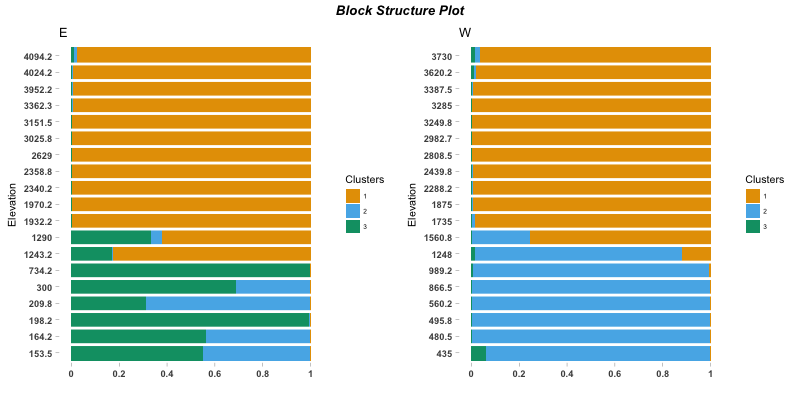
\includegraphics[width=6in,height=6in]{figure/block_structure.png}
\end{center}
\end{figure}

\newpage

\section{Processing motif data}

\section{Extras}

\textbf{ecostructure} provides additional functions for plotting a variable of interest (which could be the grades of membership or the motif pattern) against a metadata and a diversity measure or against two metadata in three way scatter plot functions.

an example of plotting a variable against two metadata are as follows.





